%% what_is_compgen.tex
%% Author: Leighton Pritchard
%% Copyright: James Hutton Institute
%% Introductory slides: What is Comparative Genomics?

% SUBSECTION
% What is Comparative Genomics?
\subsection{What is Comparative Genomics?}



%
\begin{frame}
  \frametitle{What Is Comparative Genomics?}
  Comparative genomics is$\ldots$ \\
  \Large{
    \textcolor{olive}{
      \textbf{
      The combination of genomic data, and comparative and evolutionary biology, to address questions of   genome structure, evolution, and function.
      }
    }
  }
\end{frame}

%
\begin{frame}
  \frametitle{Evolution is the central concept}
  \begin{center}
    
\includegraphics[width=\textwidth]{images/dobzhansky_quote}
  \end{center}  
\end{frame}

%
\begin{frame}
  \frametitle{Comparison of physical features}
  How do we determine that features are related, and evolved? \\
  \begin{center}
    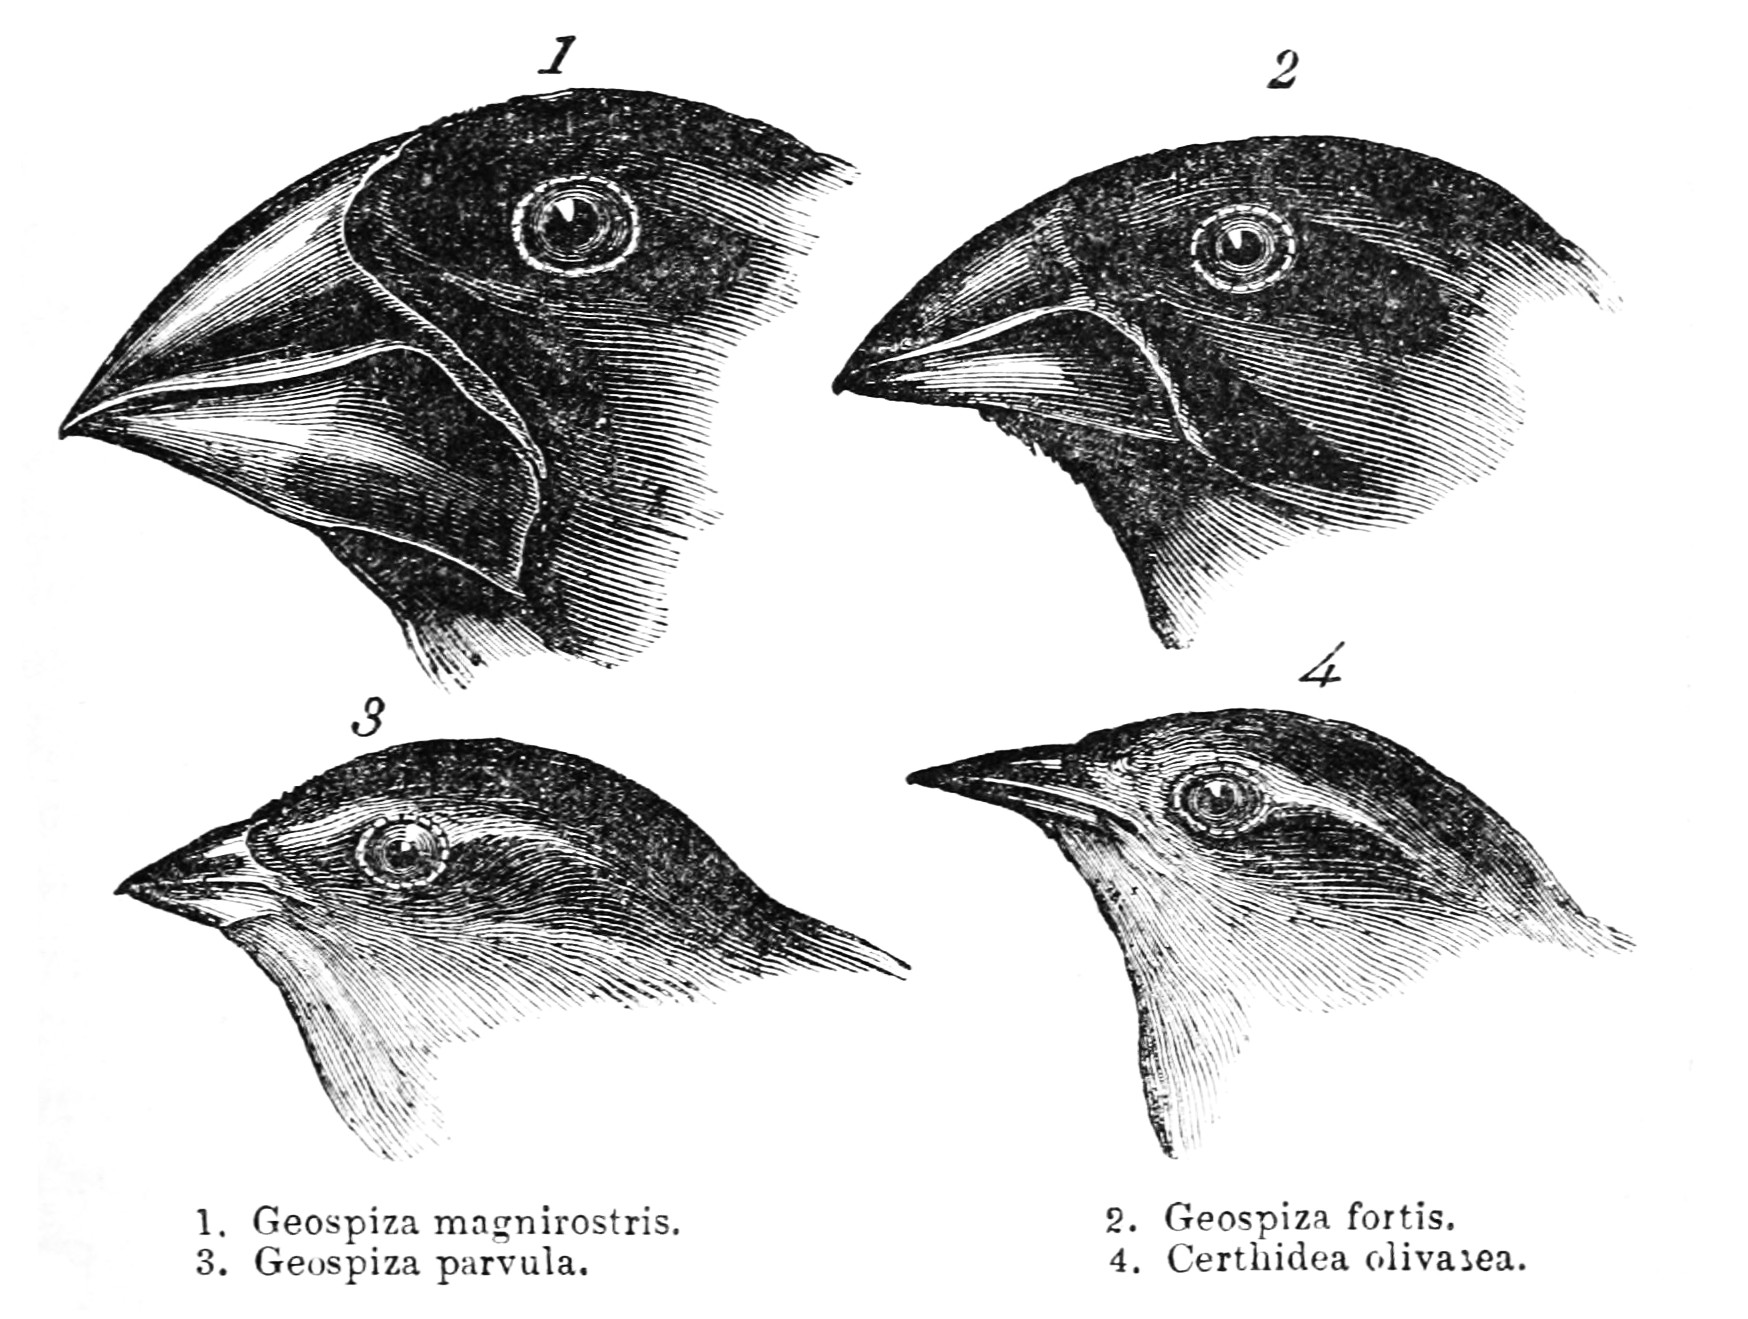
\includegraphics[width=0.8\textwidth]{images/darwin_finches}
  \end{center}  
\end{frame}

%
\begin{frame}
  \frametitle{Comparison of sequence features}
  Multiple alignment of ATP synthase \\
  \begin{center}
    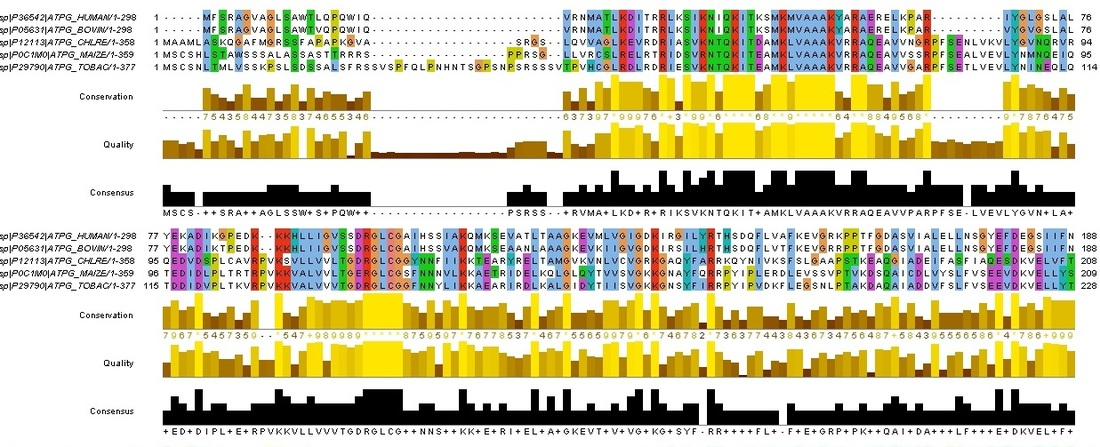
\includegraphics[width=\textwidth]{images/atp_synthase_alignment}
  \end{center}  
\end{frame}

%
\begin{frame}
  \frametitle{Comparison of genome features}
  Sequence similarity of individual features \\
  \begin{center}
    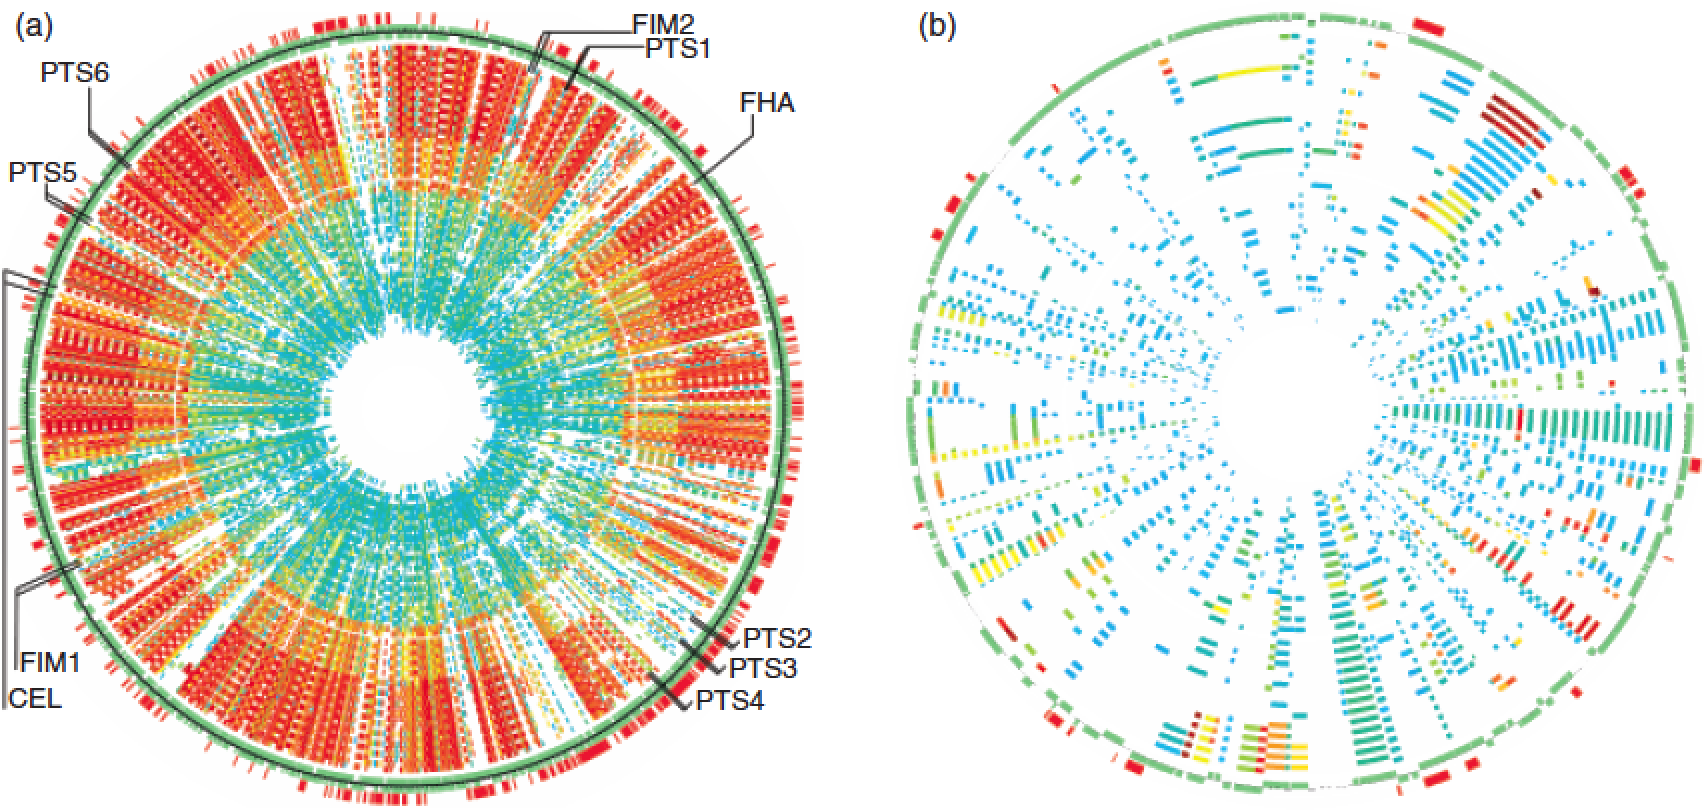
\includegraphics[width=\textwidth]{images/salmonella_circular_comparison}
  \end{center}  
\end{frame}

%
\begin{frame}
  \frametitle{Comparison of genome features}
  Genome structural rearrangements \\
  \begin{center}
    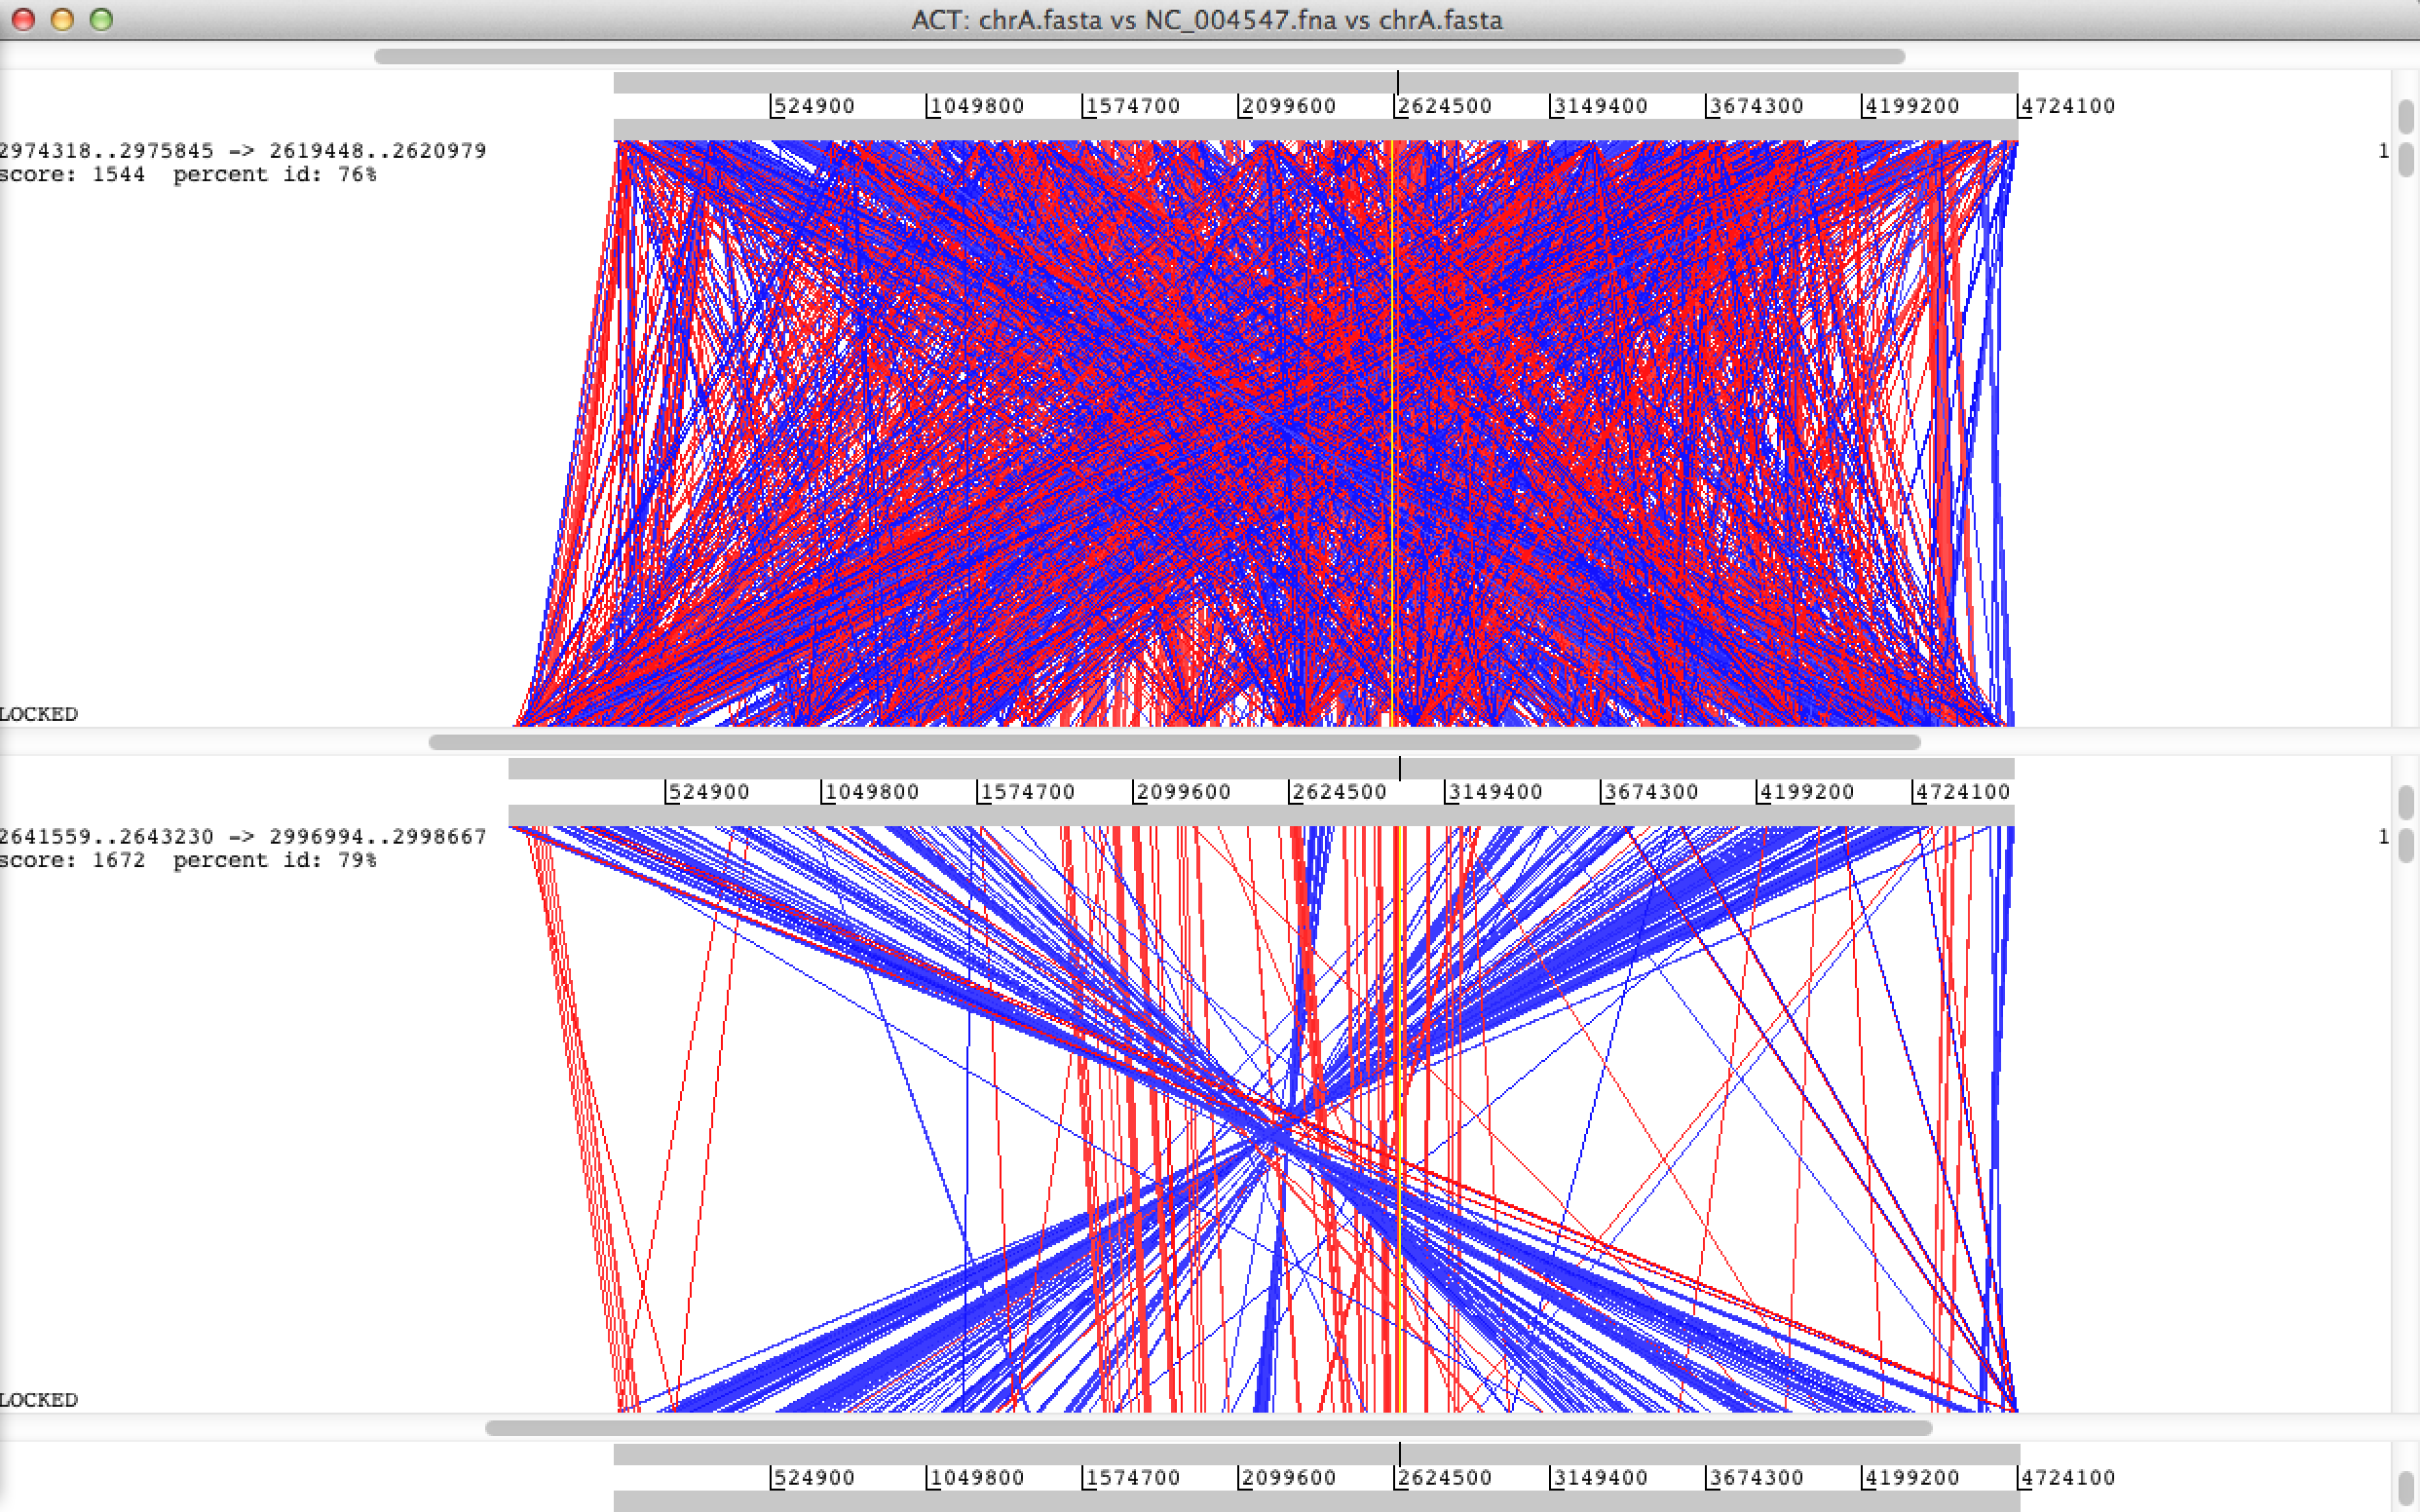
\includegraphics[width=\textwidth]{images/act_rearrangement}
  \end{center}  
\end{frame}

%
\begin{frame}
  \frametitle{Why comparative genomics?}
    \begin{columns}[c] 
      \column{.6\textwidth} 
        \begin{itemize}
         \item \textcolor{hutton_green}{Genomes describe heritable characteristics}
         \item Related organisms share ancestral genomes
         \item \textcolor{hutton_blue}{Functional elements encoded in genomes are common to related organisms}
        \end{itemize}
      \column{.4\textwidth}
        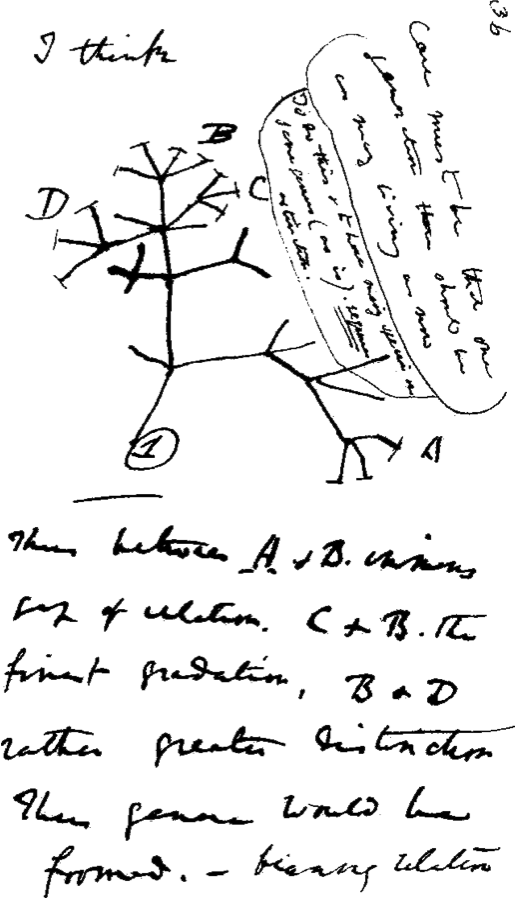
\includegraphics[width=\textwidth]{images/darwin_tree}
    \end{columns}  
\end{frame}

%
\begin{frame}
  \frametitle{Why comparative genomics?}
    \begin{columns}[c] 
      \column{.6\textwidth} 
        \begin{itemize}
         \item \textcolor{RawSienna}{Transfer of functional understanding from model systems (\textit{E. coli}, \textit{A. thaliana}, \textit{D. melanogaster}) to non-model systems}
         \item \textcolor{olive}{Genome comparisons can be informative, even for distantly-related organisms}
        \end{itemize}
      \column{.4\textwidth}
        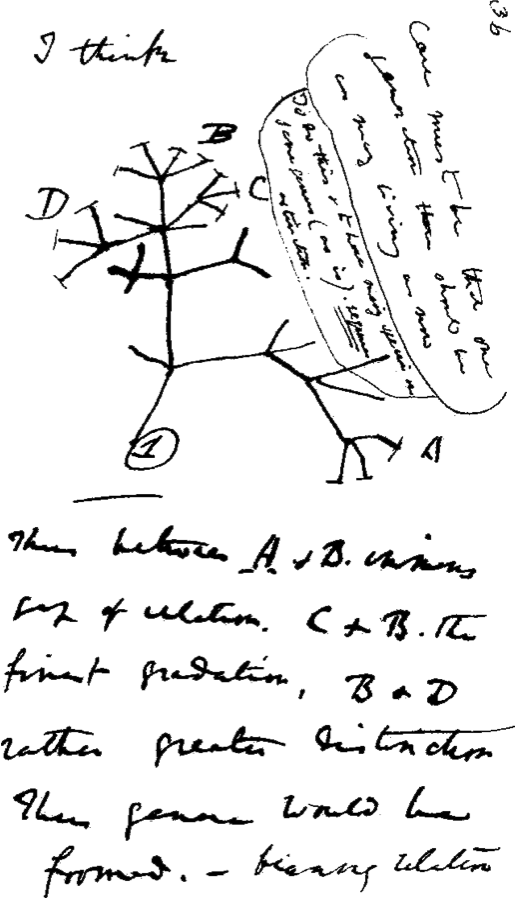
\includegraphics[width=\textwidth]{images/darwin_tree}
    \end{columns}  
\end{frame}

%
\begin{frame}
  \frametitle{Genomes are informative, but$\ldots$}
  \textcolor{hutton_blue}{\textbf{CONTEXT:}} epigenetics, tissue differentiation, mesoscale systems, etc.\\
  \begin{center}  
    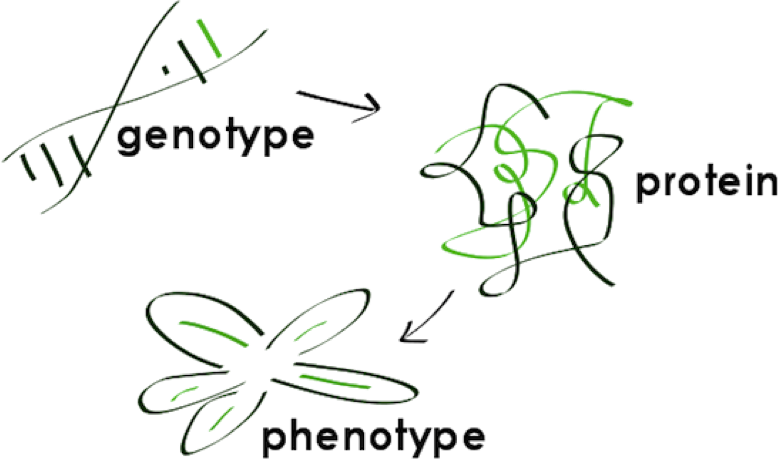
\includegraphics[width=0.7\textwidth]{images/genotype_protein_phenotype}
  \end{center}    
  \textcolor{hutton_green}{\textbf{PHENOTYPIC PLASTICITY:}} responses to temperature, stress, environment, etc.
\end{frame}

%
\begin{frame}
  \frametitle{Genomes to systems}
    \begin{columns}[c] 
      \column{.6\textwidth} 
        \textcolor{RawSienna}{\textbf{Functional Genomics}}
        \begin{itemize}
         \item \textcolor{hutton_green}{Genomic differences can underpin phenotypic (morphological or physiological) differences.}
         \item Where phenotypes/other organism-level properties are known, comparison of genomes can give mechanistic or functional insight into differences (e.g. GWAS).
         \item \textcolor{hutton_blue}{Genomic changes reveal evolutionary processes and constraints.}
        \end{itemize}
      \column{.4\textwidth}
        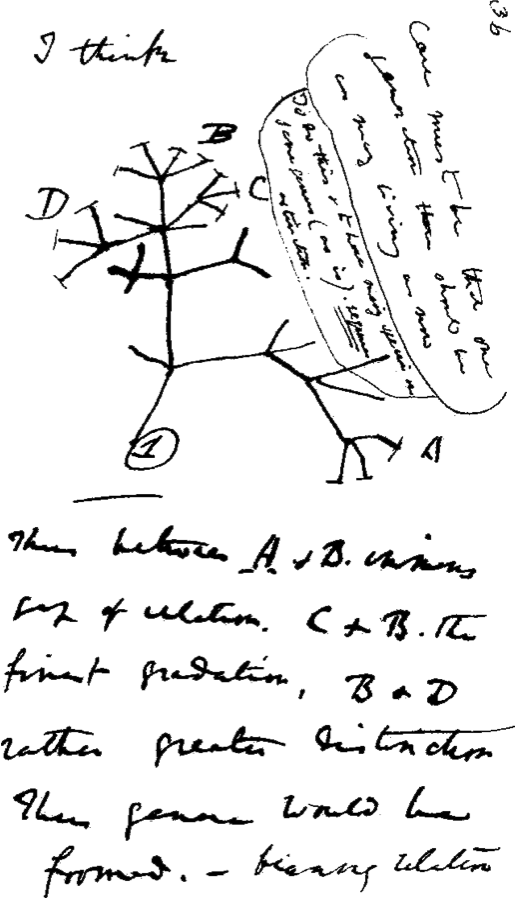
\includegraphics[width=\textwidth]{images/darwin_tree}
    \end{columns}  
\end{frame}

%
\begin{frame}
  \frametitle{\textit{E. coli} LTEE
                   \footnote{\tiny{\href{http://dx.doi.org/10.1016/j.jmb.2009.09.052
}{Jeong \textit{et al}. (2009) \textit{J. Mol. Biol.} doi:10.1016/j.jmb.2009.09.052
}}}
                   \footnote{\tiny{\href{http://dx.doi.org/10.1038/nature08480
}{Barrick \textit{et al}. (2009) \textit{Nature} doi:10.1038/nature08480
}}}
                   \footnote{\tiny{\href{http://dx.doi.org/10.1126/science.1243357
}{Wiser \textit{et al}. (2013) \textit{Science} doi:10.1126/science.1243357
}}}}
    \begin{columns}[c] 
      \column{.6\textwidth} 
        \begin{itemize}
          \item \textcolor{RawSienna}{Run by the Lenski lab, Michigan State University since 1988 \\
          (\href{http://myxo.css.msu.edu/ecoli/}{http://myxo.css.msu.edu/ecoli/})}
          \item \textcolor{hutton_green}{12 flasks, citrate usage selection}
          \item \textcolor{hutton_blue}{$>$50,000 generations of \textit{E coli}!}
          \begin{itemize}
            \item Cultures propagated every day
            \item Every 500 generations (75 days), mixed-population samples stored
            \item Mean fitness estimated at 500 generation intervals
          \end{itemize}
        \end{itemize}
      \column{.4\textwidth}
        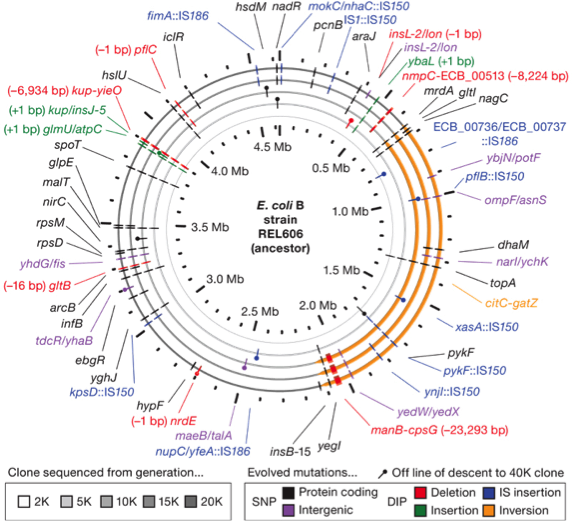
\includegraphics[width=\textwidth]{images/ltee_circular} \\
        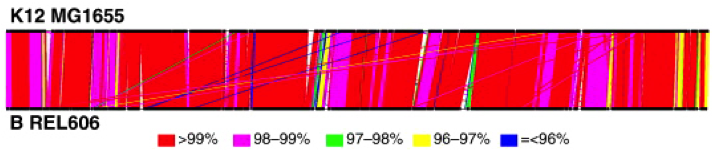
\includegraphics[width=\textwidth]{images/ltee_linear}        
    \end{columns}  
\end{frame}

%
\begin{frame}
  \frametitle{Comparative genomics in the news
                   \footnote{\tiny{\href{http://www.washingtonpost.com/news/speaking-of-science/wp/2015/02/23/the-mysterious-genes-of-carnivorous-bladderwort-reveal-themselves/
}{Washington Post 23/2/2015
}}}
                   \footnote{\tiny{\href{http://dx.doi.org/10.1038/nature12132
}{Ibarra-Laclette \textit{et al}. (2013) \textit{Nature} doi:10.1038/nature12132
}}}
                   \footnote{\tiny{\href{http://dx.doi.org/10.1093/molbev/msv020
}{Carretero-Paulet \textit{et al}. (2015) \textit{Mol. Biol. Evol.} doi:10.1093/molbev/msv020
}}}
}
    \begin{columns}[c] 
      \column{.6\textwidth} 
        \begin{itemize}
          \item \textcolor{RawSienna}{\textit{Utricularia gibba}: carnivorous bladderwort}
          \item \textcolor{hutton_blue}{Genome: 82Mbp, 17,324 genes \\
          (wheat: 17bn bases, $\approx$94-96k genes)}
          \item Intergenic region contraction \\
          (3\% repeat elements; most plants: 10-60\% repeat elements)
          \item \textcolor{hutton_green}{Genomic context for flowering plants does not require ``hidden regulators'' (cf. ENCODE)}
        \end{itemize}
      \column{.4\textwidth}
        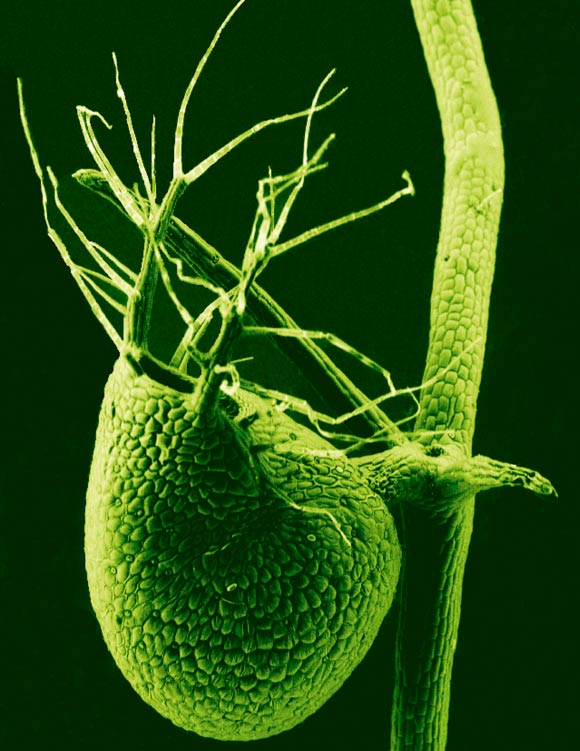
\includegraphics[height=0.3\textheight]{images/Utricularia-gibba}
        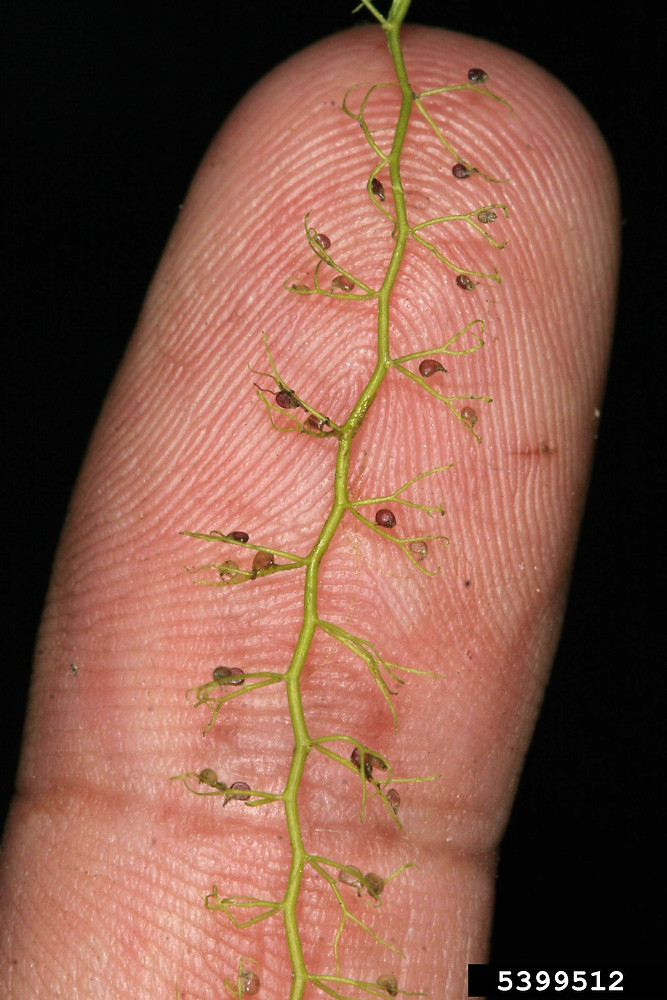
\includegraphics[height=0.3\textheight]{images/utricularia-gibba-finger} \\
        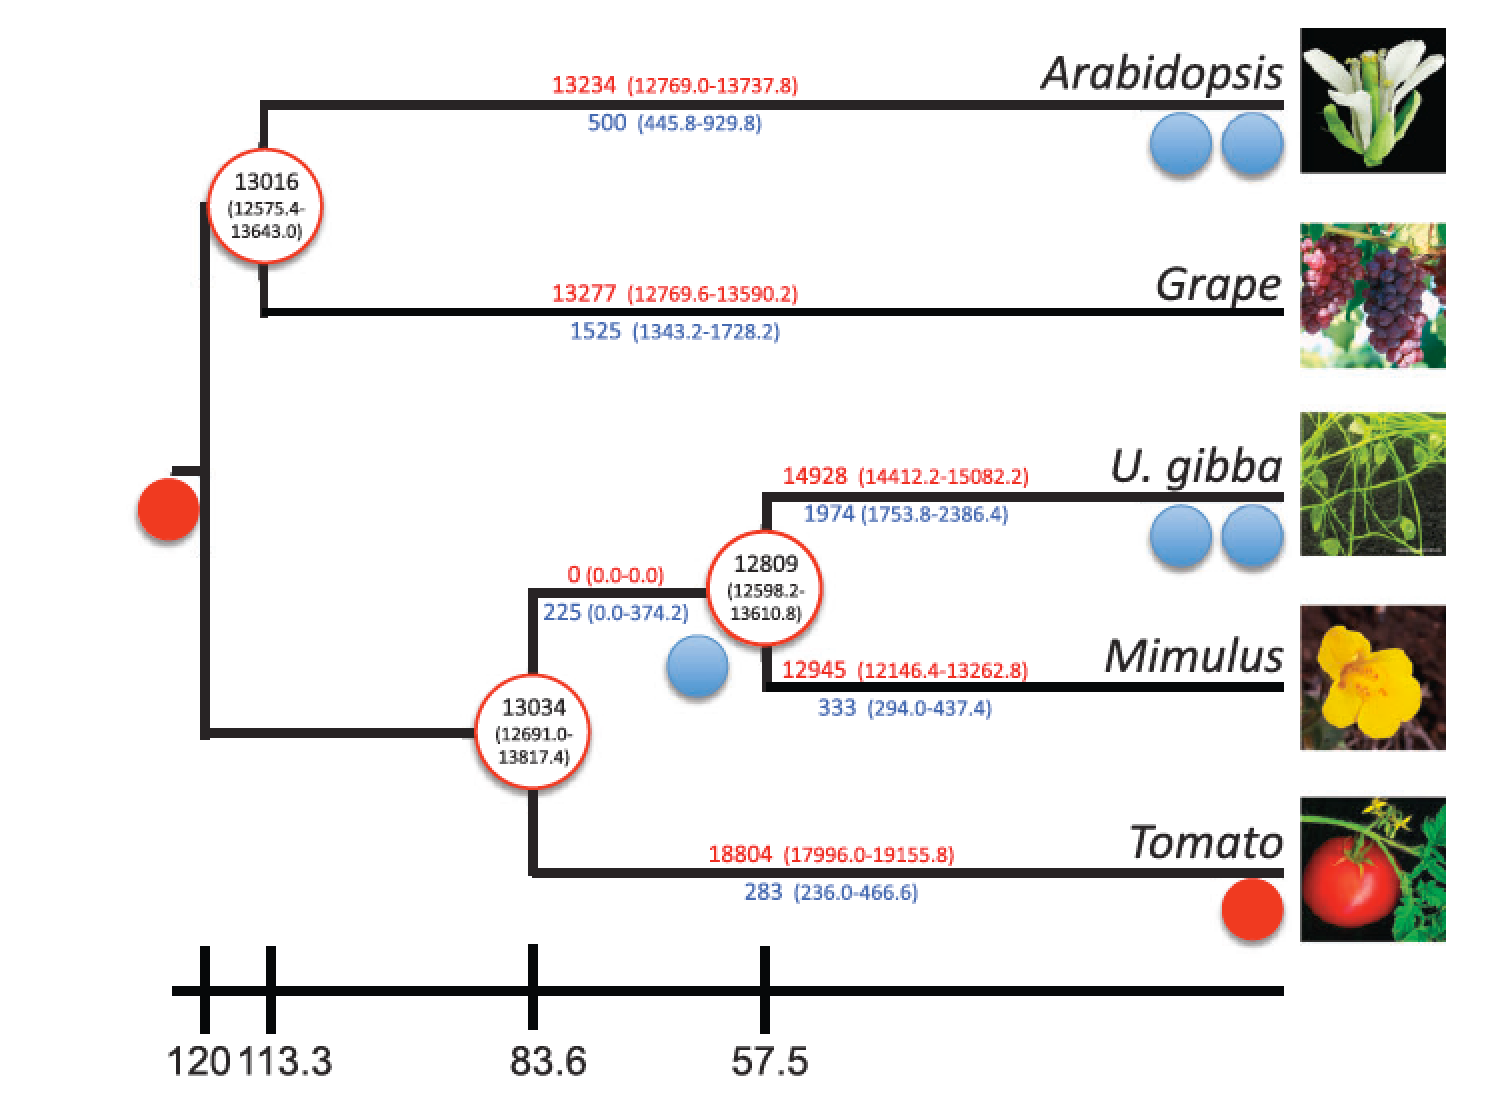
\includegraphics[width=\textwidth]{images/U_gibba_tree}        
    \end{columns}  
\end{frame}